\section{Experiments}

\paragraph{Datasets.}
We evaluate on three multi-batch single-cell RNA-seq datasets~\citep{luecken2020benchmarking}:
\textbf{Pancreas} (16,382 cells, 9 technologies, 14 cell types),
\textbf{PBMC (immune)} (30k cells, 5 batches, 9 cell types),
and a \textbf{Lung} dataset (30k cells, 16 batches, 17 cell types).
For spatial evaluations, we use a \textbf{non-small cell lung cancer (NSCLC)} spatial transcriptomics dataset~\citep{pentimalli2025combining}.
The original dataset comprises 6 slides; we select slide 28, subsample 30,000 cells stratified by cell type and niche label, and exclude cells assigned to uninformative niche labels, yielding 28,804 cells across 18 cell types and 9 niches.
All datasets are preprocessed with Scanpy~\citep{wolf2018scanpy} by normalizing total counts, applying log1p transformation, and selecting 4,000 highly variable genes.
Detailed statistics are in Appendix~\ref{app:datasets}.

\paragraph{Affinity construction.}
For transcriptomic experiments, cell--cell affinities are computed using an adaptive Gaussian kernel on PCA embeddings, following prior work~\citep{seacells}.
For spatial experiments, we apply the same kernel to spatially aggregated features, obtained by averaging the PCA embeddings of neighboring cells within a fixed spatial radius, thereby incorporating microenvironmental context into the affinity.

\paragraph{Baselines.}
We compare against \textbf{SEACells}~\citep{seacells}, a metacell method based on archetypal analysis;
\textbf{CVAE}, a reconstruction-only variant without affinity guidance, isolating the effect of the affinity loss;
and \textbf{Parametric UMAP}, which preserves data geometry by aligning pairwise relationships in the embedding space.
Since CVAE and Parametric UMAP do not produce discrete cluster assignments, we apply $K$-means clustering on their learned embedding spaces to obtain metacells, using the same $K$ as scProto.
For spatial experiments, we additionally evaluate \textbf{SEACells (spatial)}, trained on the same spatial affinity graph as scProto.

\paragraph{Evaluation protocol.}
scProto outputs soft prototype assignments $s_i \in \mathbb{R}^K$; each cell is assigned to the prototype with the highest assignment score (argmax), and each metacell is labeled by majority voting over its assigned cells.
We evaluate through a sequence of analyses aligned with the model's design goals.
First, we assess whether learned metacells respect the community structure of the input affinity graph using \textbf{modularity}, computed on per-batch subgraphs (all edges incident to at least one cell in the batch); mean and standard deviation are reported across batches.
Second, we evaluate cross-batch aggregation by measuring \textbf{batch entropy} of each metacell, defined as the Shannon entropy of its batch label distribution: $H(m) = -\sum_b p_b \log p_b$, where $p_b$ is the fraction of cells in metacell $m$ from batch $b$.
Third, we examine whether cross-batch alignment preserves biological signal using \textbf{cell-type purity}, defined as the fraction of cells in a metacell belonging to the most frequent cell type: $\text{purity}(m) = \frac{1}{|m|} \max_{c} \sum_{i \in m} \mathbf{1}[y_i = c]$.
We then focus on underrepresented populations, measuring \textbf{coverage}---whether each rare cell type is represented by at least one metacell---and \textbf{rare purity}, where rare cell types are defined as the bottom 25th percentile by frequency.
For spatial data, we additionally evaluate \textbf{niche purity} alongside cell-type purity to assess capture of microenvironmental structure.

\subsection{scProto recovers community structure while integrating cells across batches}

As shown in Table~\ref{tab:graph_batch}, scProto achieves modularity comparable to SEACells, indicating that it recovers the community structure of the input affinity graph. At the same time, it exhibits substantially higher batch entropy, demonstrating effective mixing of cells across batches. Importantly, this is achieved without compromising biological identity, as scProto maintains cell-type purity comparable to competing methods.

In contrast, SEACells attains similar modularity and purity but exhibits very low batch entropy, indicating that it forms batch-specific metacells without meaningful cross-batch aggregation. Conversely, CVAE and parametric UMAP achieve high batch entropy and purity but show significantly lower modularity, suggesting that they fail to recover the community structure encoded in the affinity graph.

These differences are further illustrated in Fig.~\ref{fig:pancreas_umap}, where UMAP~\citep{mcinnes2018umap} visualizations of pancreas metacells show that scProto forms clusters that are well aligned across batches while remaining consistent with cell-type structure, whereas SEACells produces clusters that are largely separated by batch.
Per-metacell distributions of purity and batch entropy are shown in Fig.~\ref{fig:purity_entropy} (Appendix).

\begin{figure*}[t]
\centering
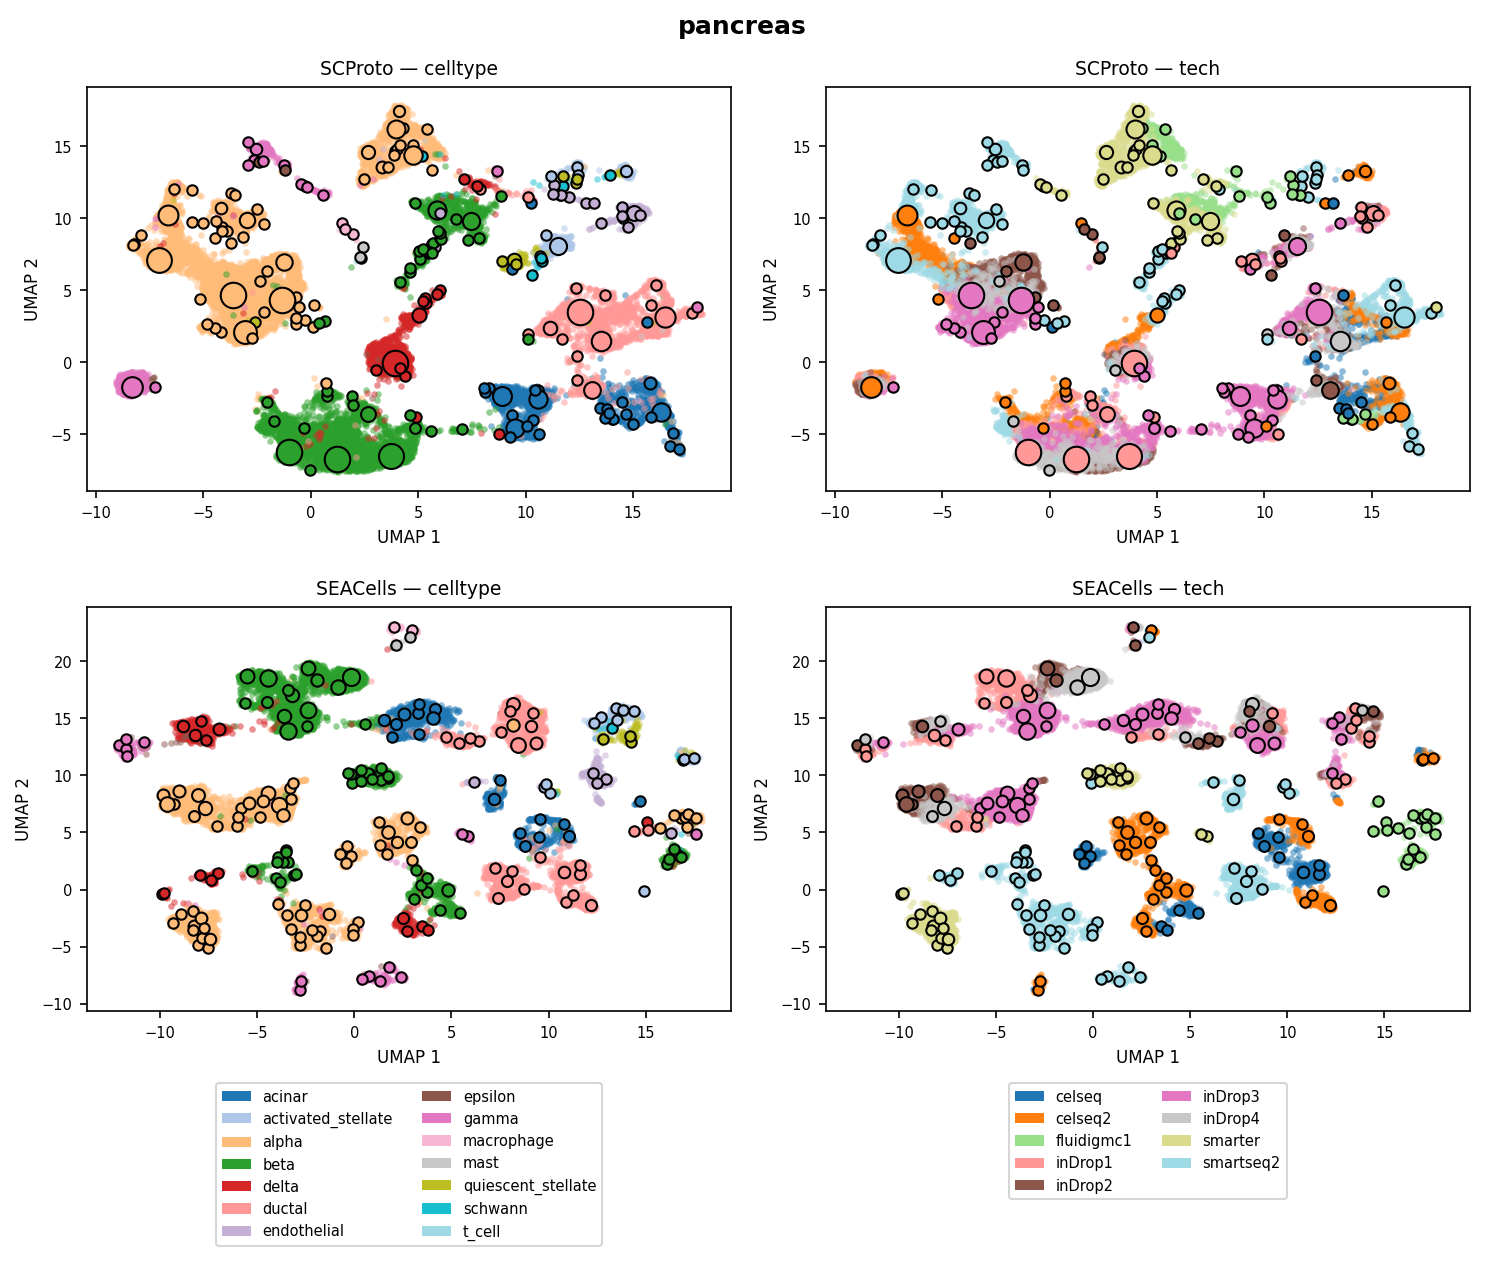
\includegraphics[width=\textwidth]{figures/pancreas_umap.png}
\caption{
UMAP visualization of metacells on the Pancreas dataset.
Top: scProto. Bottom: SEACells.
Left: colored by cell type. Right: colored by batch (technology).
scProto forms compact, biologically coherent clusters while mixing cells across batches.
SEACells produces batch-specific, fragmented metacells.
Black circles denote metacells (size proportional to number of assigned cells).
}
\label{fig:pancreas_umap}
\end{figure*}

\begin{table*}[t]
\centering
\caption{Community structure preservation and cross-batch integration performance.
Modularity is computed on per-batch subgraphs; batch entropy and purity are computed per metacell.
All values are reported as mean~$\pm$~std across batches (modularity) or across metacells (entropy, purity); variability therefore reflects the distribution over metacells within each dataset.
Best results are in bold and second-best results are underlined.}
\label{tab:graph_batch}
\tiny
\setlength{\tabcolsep}{1pt}
\begin{tabular}{lccc|ccc|ccc}
\toprule
 & \multicolumn{3}{c}{Pancreas}
 & \multicolumn{3}{c}{Immune}
 & \multicolumn{3}{c}{Lung} \\
\cmidrule(lr){2-4} \cmidrule(lr){5-7} \cmidrule(lr){8-10}
Method
& Modularity $\uparrow$ & Batch Entropy $\uparrow$ & Purity $\uparrow$
& Modularity $\uparrow$ & Batch Entropy $\uparrow$ & Purity $\uparrow$
& Modularity $\uparrow$ & Batch Entropy $\uparrow$ & Purity $\uparrow$ \\
\midrule

SEACells
& $\mathbf{0.67 \pm 0.05}$ & $0.19 \pm 0.30$ & $\underline{0.97 \pm 0.08}$
& $\underline{0.55 \pm 0.04}$ & $0.16 \pm 0.24$ & $\mathbf{0.88 \pm 0.14}$
& $\mathbf{0.67 \pm 0.04}$ & $0.41 \pm 0.47$ & $\mathbf{0.90 \pm 0.15}$ \\

MetaQ
& $0.41 \pm 0.10$ & $0.38 \pm 0.41$ & $0.96 \pm 0.11$
& $0.28 \pm 0.11$ & $0.63 \pm 0.50$ & $0.81 \pm 0.15$
& $0.42 \pm 0.14$ & $0.53 \pm 0.54$ & $0.91 \pm 0.13$ \\

CVAE
& $0.23 \pm 0.07$ & $\underline{1.38 \pm 0.41}$ & $0.97 \pm 0.07$
& $0.26 \pm 0.14$ & $0.81 \pm 0.40$ & $0.87 \pm 0.14$
& $0.32 \pm 0.05$ & $\underline{1.33 \pm 0.43}$ & $0.86 \pm 0.18$ \\

UMAP
& $0.26 \pm 0.06$ & $\mathbf{1.51 \pm 0.37}$ & $0.94 \pm 0.10$
& $0.26 \pm 0.14$ & $0.80 \pm 0.40$ & $0.87 \pm 0.15$
& $0.32 \pm 0.06$ & $1.32 \pm 0.44$ & $0.86 \pm 0.18$ \\

\midrule

scProto
& $\underline{0.61 \pm 0.08}$ & $1.04 \pm 0.66$ & $\mathbf{0.98 \pm 0.07}$
& $\mathbf{0.62 \pm 0.08}$ & $\underline{0.94 \pm 0.51}$ & $0.87 \pm 0.13$
& $\mathbf{0.67 \pm 0.03}$ & $\mathbf{1.39 \pm 0.55}$ & $0.86 \pm 0.18$ \\

\bottomrule
\end{tabular}
\setlength{\tabcolsep}{6pt}
\end{table*}

\subsection{Cross-Batch Metacells Improve Representation of Rare Cell Types}

We next examine whether cross-batch aggregation improves the representation of low-frequency (rare) cell types.

As shown in Table~\ref{tab:rare_cells}, scProto achieves consistently higher or comparable coverage across datasets, indicating that aggregating cells across batches enables the formation of metacells for cell types that are underrepresented within individual batches. Importantly, scProto also attains higher or comparable purity for metacells corresponding to rare cell types, demonstrating that it groups cells more coherently despite limited per-batch samples.

To further analyze performance across the frequency spectrum, we stratify cell types by frequency and evaluate metacell purity within each bin (Fig.~\ref{fig:rare_purity}, Appendix). scProto maintains high purity even for the rarest cell types, whereas SEACells shows a noticeable degradation in low-frequency bins. This suggests that restricting aggregation within batches limits the ability to form reliable metacells when only few samples are available per batch.

In contrast, reconstruction-based methods such as CVAE, and structure-preserving methods such as parametric UMAP, do not explicitly enforce community-level structure during training. As a result, they tend to merge rare cell states into larger, denser clusters, leading to reduced purity for low-frequency populations.


\begin{table*}[t]
\centering
\caption{Performance on rare cell types.
We report cell-type coverage (higher is better) and cell-type purity for low-frequency (rare) cell types (higher is better).
Purity values are reported as mean~$\pm$~std across metacells assigned to rare cell types; variability reflects the distribution over those metacells.
Best results are in bold and second-best results are underlined.}
\label{tab:rare_cells}
\tiny
\begin{tabular}{lcc|cc|cc}
\toprule
 & \multicolumn{2}{c}{Pancreas}
 & \multicolumn{2}{c}{Immune}
 & \multicolumn{2}{c}{Lung} \\
\cmidrule(lr){2-3} \cmidrule(lr){4-5} \cmidrule(lr){6-7}
Method
& Coverage $\uparrow$
& Rare Purity $\uparrow$
& Coverage $\uparrow$
& Rare Purity $\uparrow$
& Coverage $\uparrow$
& Rare Purity $\uparrow$ \\
\midrule

SEACells
& $0.50$ & $0.69 \pm 0.11$
& $\mathbf{1.00}$ & $\mathbf{0.90 \pm 0.10}$
& $\mathbf{1.00}$ & $\underline{0.92 \pm 0.13}$ \\

MetaQ
& $0.25$ & $\underline{0.71 \pm 0.00}$
& $\mathbf{1.00}$ & $0.78 \pm 0.05$
& $0.00$ & -- \\

CVAE
& $\underline{0.75}$ & $0.54 \pm 0.09$
& $0.75$ & $0.58 \pm 0.21$
& $\underline{0.67}$ & $0.82 \pm 0.13$ \\

UMAP
& $0.50$ & $0.55 \pm 0.15$
& $\mathbf{1.00}$ & $0.61 \pm 0.12$
& $\mathbf{1.00}$ & $0.84 \pm 0.18$ \\

\midrule

scProto
& $\mathbf{1.00}$ & $\mathbf{0.73 \pm 0.13}$
& $\mathbf{1.00}$ & $\underline{0.88 \pm 0.13}$
& $\mathbf{1.00}$ & $\mathbf{0.95 \pm 0.09}$ \\

\bottomrule
\end{tabular}
\end{table*}

\subsection{scProto captures microenvironmental and spatial structure}

We evaluate whether incorporating spatial information enables scProto to capture microenvironmental structure while preserving cell-type identity.

As shown in Fig.~\ref{fig:spatial_heatmap}, scProto achieves a strong balance between cell-type purity and niche purity, indicating that it captures spatially relevant structure without compromising biological identity. In contrast, SEACells trained on transcriptomic similarity fails to capture spatial organization, resulting in low niche purity. While SEACells trained on spatial affinity improves niche purity, it does so at the expense of cell-type purity, suggesting a loss of biological specificity.
\begin{figure*}[t]
\centering
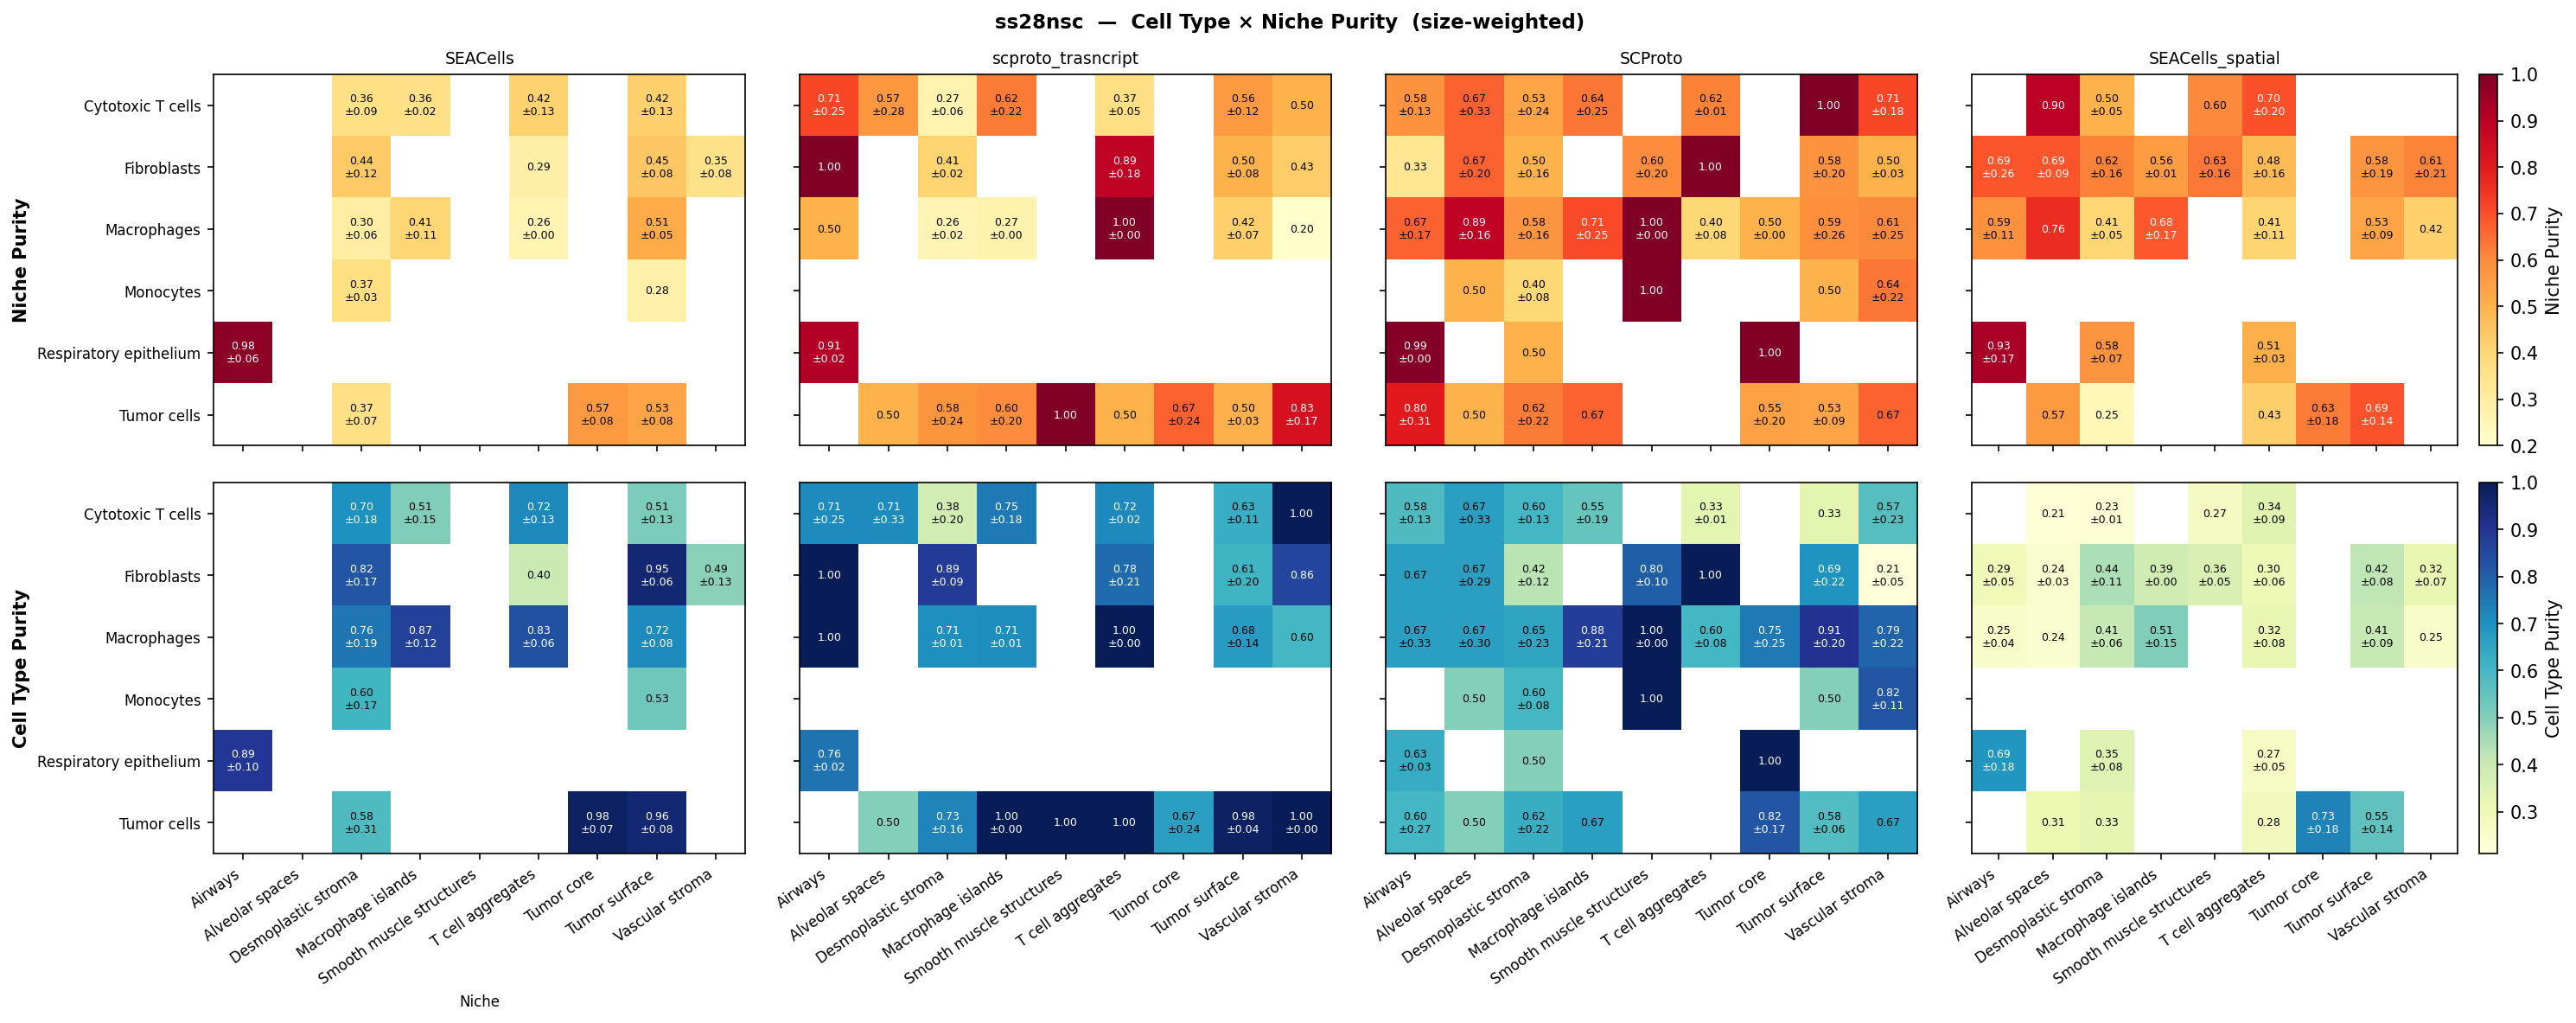
\includegraphics[width=\textwidth]{figures/heatmap.png}
\caption{
Cell type-- and niche-specific evaluation of niche purity and cell-type purity using size-weighted metrics.
Each entry shows mean $\pm$ standard deviation across metacells.
}
\label{fig:spatial_heatmap}
\end{figure*}

These differences are further illustrated in Fig.~\ref{fig:spatial} (Appendix), where spatial visualizations show that scProto groups cells from the same niches while maintaining coherent cell-type structure. This indicates that incorporating spatial affinity enables scProto to capture gene expression patterns associated with microenvironmental context---signals that are not recoverable from transcriptomic similarity alone.


% \begin{figure*}[t]
% \centering
% 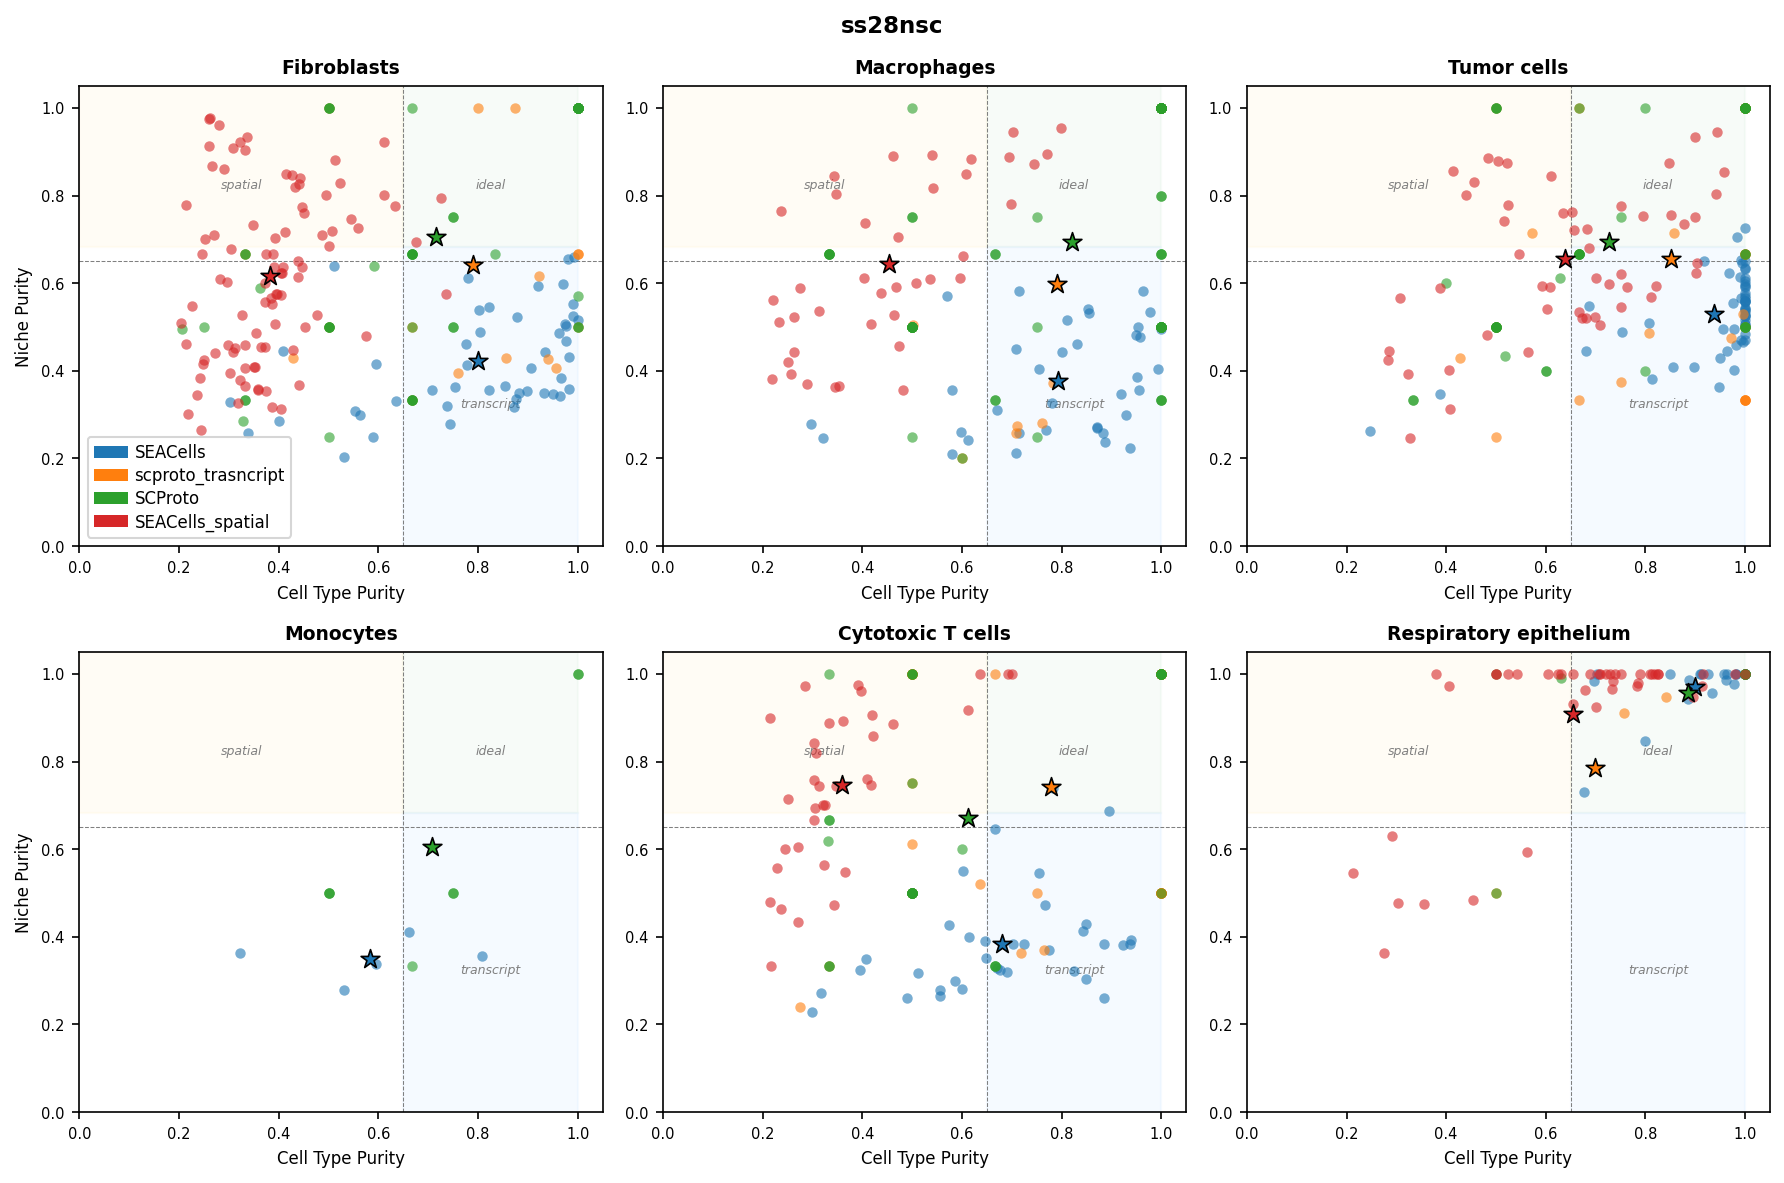
\includegraphics[width=\textwidth]{figures/tradeoff.png}
% \caption{
% Trade-off between cell-type purity and niche purity across metacells.
% Each point represents a metacell, colored by method, and star markers indicate method centroids.
% Arrows indicate the effect of incorporating spatial context by comparing scProto trained on transcriptomic similarity with scProto trained on spatial similarity.
% }
% \label{fig:spatial_tradeoff}
% \end{figure*}

% \begin{figure*}[t]
% \centering
% 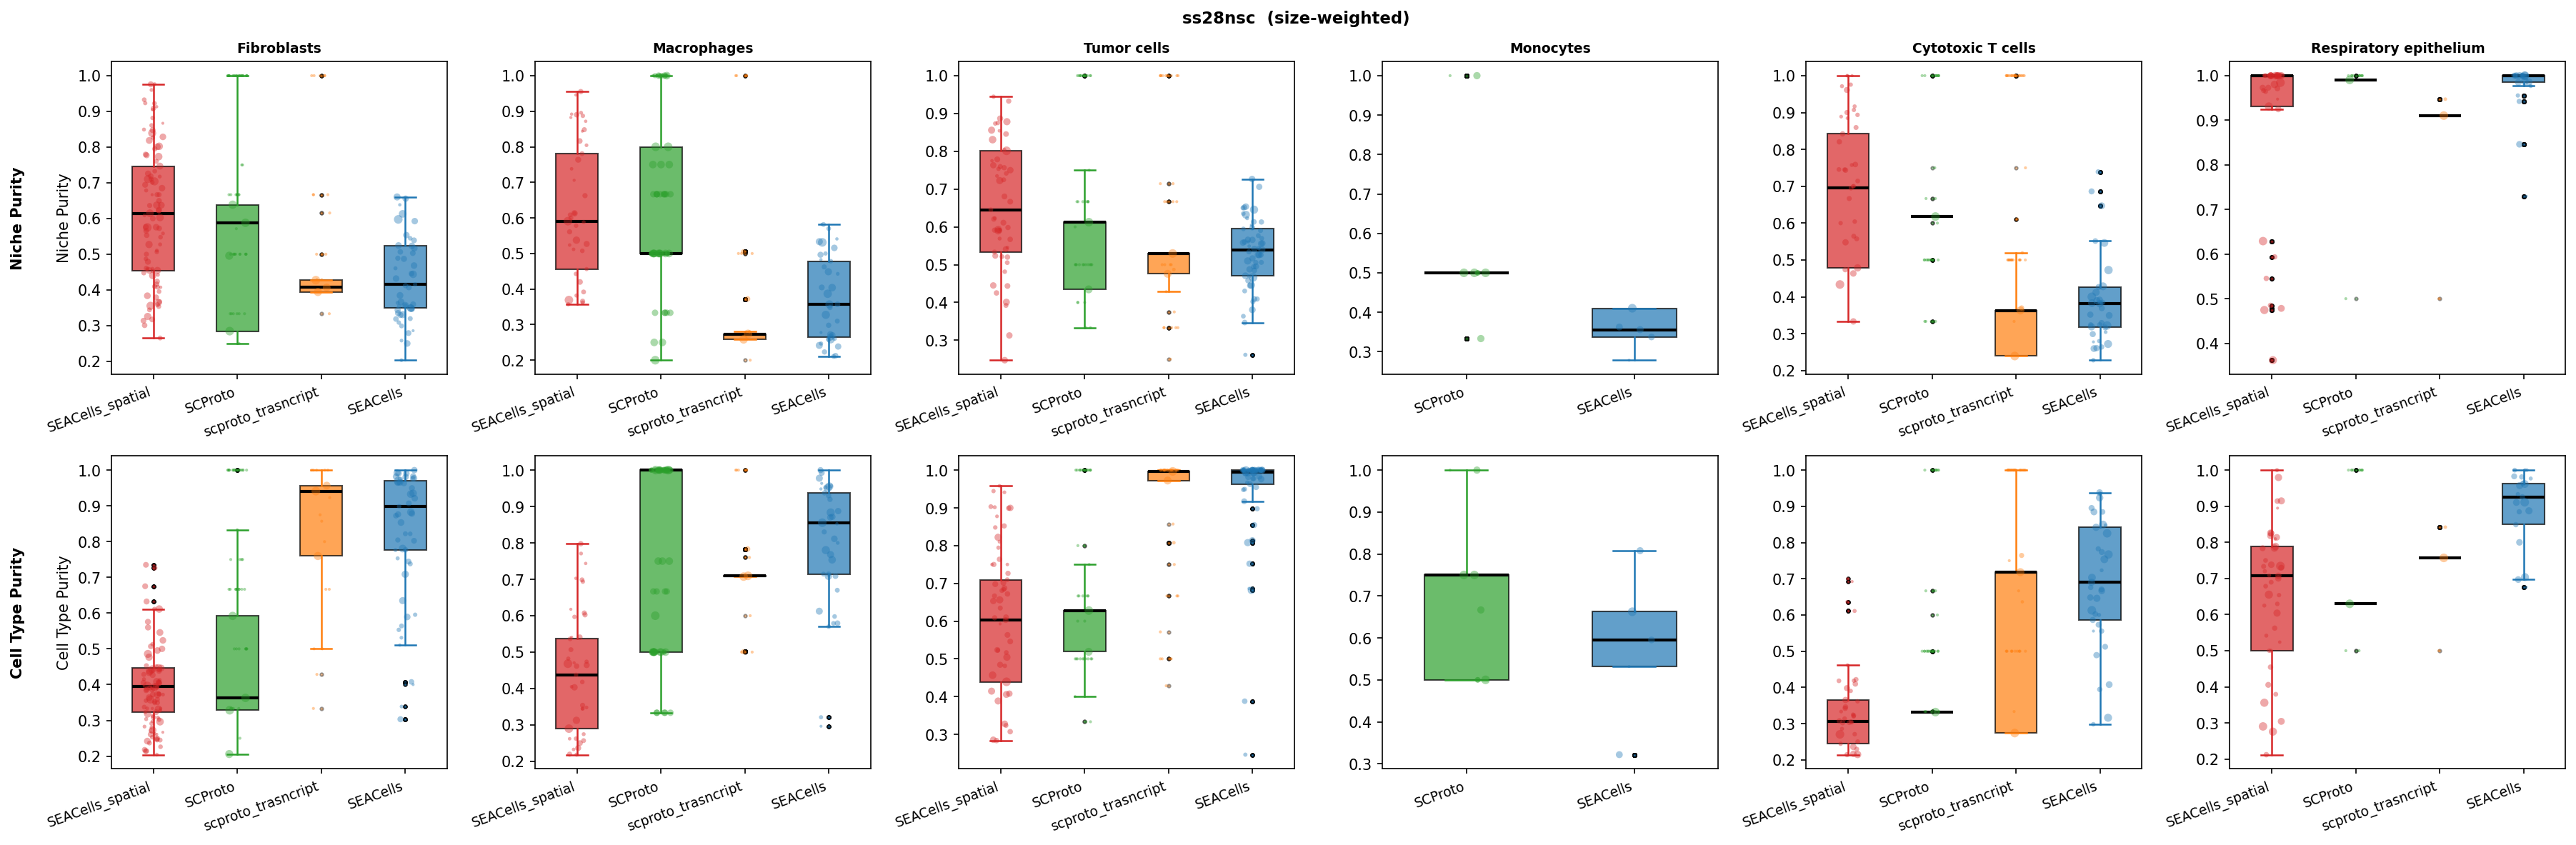
\includegraphics[width=\textwidth]{figures/niche_box.png}
% \caption{
% Comparison of niche purity and cell-type purity across methods for selected cell types using size-weighted metrics.
% scProto improves niche purity compared to transcriptomics-only methods while maintaining substantially higher cell-type purity than the spatial SEACells baseline.
% }
% \label{fig:spatial_boxplots}
% \end{figure*}
